
%\RequirePackage{pdf15}

\documentclass{beamer}

\usepackage[utf8]{inputenc}

\usepackage{mystyle}

\usepackage{tikz}
\usepackage{pgfplots}
\usepackage{subcaption}

%\usepackage{natbib}
\usepackage[style=authortitle,backend=biber]{biblatex}
\addbibresource{anthology.bib}
\addbibresource{emnlp2020.bib}
\renewcommand{\footnotesize}{\scriptsize}

\usepackage{tikz-dependency}
\usetikzlibrary{shapes.arrows, positioning, fit, bayesnet,
    arrows,backgrounds,patterns,matrix,calc,shadows,plotmarks,
    shapes,positioning,automata,positioning,spy,scopes,chains,decorations,decorations.pathreplacing}

\newcommand{\FancyUpArrow}{
\begin{tikzpicture}[baseline=-0.3em]
\node[single arrow,draw,rotate=90,single arrow head extend=0.2em,inner
ysep=0.2em,transform shape,line width=0.05em,top color=green,bottom color=green!50!black] (X){};
\end{tikzpicture}}
\newcommand{\FancyDownArrow}{
\begin{tikzpicture}[baseline=-0.3em]
\node[single arrow,draw,rotate=-90,single arrow head extend=0.2em,inner
ysep=0.2em,transform shape,line width=0.05em,top color=red,bottom color=red!50!black] (X){};
\end{tikzpicture}}

\AtBeginSection[]{
  \begin{frame}
  \vfill
  \centering
  \begin{beamercolorbox}[sep=8pt,center,shadow=true,rounded=true]{title}
    \usebeamerfont{title}\insertsectionhead\par%
  \end{beamercolorbox}
  \vfill
  \end{frame}
}

% quotes
\usepackage[style=british]{csquotes}

\def\signed #1{{\leavevmode\unskip\nobreak\hfil\penalty50\hskip1em
  \hbox{}\nobreak\hfill #1%
  \parfillskip=0pt \finalhyphendemerits=0 \endgraf}}

\newsavebox\mybox
\newenvironment{aquote}[1]
  {\savebox\mybox{#1}\begin{quote}\openautoquote\hspace*{-.7ex}}
  {\unskip\closeautoquote\vspace*{1mm}\signed{\usebox\mybox}\end{quote}}

%Information to be included in the title page:
\title{Low-Rank Constraints for Fast Inference in Structured Models}
\author{Justin Chiu* and Yuntian Deng* and Alexander Rush}

\setbeamertemplate{navigation symbols}{} 
\setbeamertemplate{footline}[frame number]

\begin{document}

\begin{frame}[plain]
\titlepage
\end{frame}

\begin{frame}
\frametitle{Structured Models}
\begin{itemize}
\item Explicitly model output associations
\vspace{1em}
    \begin{itemize}
    \item Directly or through \underline{latent variables}
    \end{itemize}
\vspace{1em}
\item Focus on combinatorially large latent \underline{discrete structures}
\vspace{1em}
    \begin{itemize}
    \item Complementary to distributed representations
    \end{itemize}
\end{itemize}
\end{frame}

\begin{frame}
\frametitle{Scaling Structured Models}

\begin{itemize}
\item Prior work demonstrated: Size \FancyUpArrow ~ Performance \FancyUpArrow
    \begin{itemize}
    \item Hidden Markov Models (HMM)
    \item Probabilistic Context-Free Grammars (PCFG)
    \end{itemize}
\vspace{1em}
\item Prior work scaled via
    \begin{itemize}
    \item Sparsity for HMMs \footcite{chiu2020hmm}
    \item Low-rank tensor decompositions for PCFGs \footcite{yang2021pcfg}
    \end{itemize}
    \vspace{1em}
\item This work: low-rank matrix constraints
    \begin{itemize}
    \item More general
    \item Less speedup
    \end{itemize}
\end{itemize}
\end{frame}

\begin{frame}
\frametitle{Inference as Matrix-Vector Products}
\begin{itemize}
\item Inference: sequence of matrix-vector products
\vspace{1em}
\item Speed up via fast mat-vecs 
\vspace{1em}
\item Applies to a large family of structured models
\end{itemize}
\end{frame}

\begin{frame}
\frametitle{Fast Matrix-Vector Products}
\begin{itemize}
\item Mat-vecs take $O(L^2)$ computation
\vspace{1em}
\item Various fast methods
    \begin{itemize}
    \item Sparsity (nnz entries)
    \item Fast Fourier Transform ($L \log L$)
    \item \underline{Low-Rank factorization} ($LR$)
    \end{itemize}
\vspace{1em}
\item Connected to work in efficient attention and low-dimensional kernel approximations
\footcite{performer,rfa,blanc2018adaptive}
\end{itemize}
\end{frame}

\begin{frame}
\frametitle{Roadmap}
\begin{itemize}
\item Speeding up HMM inference
\vspace{1em}
\item Speeding up PCFG inference
\vspace{1em}
\item Generalization to hypergraph inference
\vspace{1em}
\item Experiments
\end{itemize}
\end{frame}

\begin{frame}
\frametitle{Two Examples}
\begin{columns}
\begin{column}{0.5\textwidth}
   some text here some text here some text here some text here some text here
\end{column}
\hspace{-50pt}
\vrule{}
\begin{column}{0.5\textwidth}  %%<--- here
    \begin{itemize}
        \item Blah
    \end{itemize}
\end{column}
\end{columns}
\end{frame}

\begin{frame}
\frametitle{Hidden Markov Models (HMMs)}

For times $t$, model states $z_t \in [Z]$, and tokens $x_t \in [X]$,

\vspace{1em}

\begin{center}
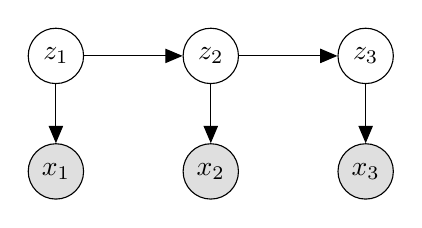
\begin{tikzpicture}[]
\node[latent] (z0) {$z_1$} ;
\node[latent] (z1) [right=1.25cm of z0] {$z_2$} ;
\node[latent] (z2) [right=1.25cm of z1] {$z_3$} ;

\node[obs]    (x0) [below = 0.75cm of z0] {$x_1$};
\node[obs]    (x1) [below = 0.75cm of z1] {$x_2$};
\node[obs]    (x2) [below = 0.75cm of z2] {$x_3$};

\edge {z0} {x0};
\edge {z1} {x1};
\edge {z2} {x2};
\edge {z0} {z1};
\edge {z1} {z2};
\end{tikzpicture}
\end{center}

\vspace{1em}
with joint distribution
$$p(x,z) = \prod_t p(x_t \mid z_t)p(z_t \mid z_{t-1})$$
\end{frame}

\begin{frame}
\frametitle{Inference}
Given observed $x = (x_1, \ldots, x_T)$
\vspace{1em}
We wish to maximize
\begin{equation*}
p(x)
= \sum_{z_1}\cdots\sum_{z_T}p(x, z)
= \alpha_1^\top\Lambda_2\Lambda_3\cdots\Lambda_T\bm1,
\end{equation*}
where we have the
\begin{align*}
&\textnormal{start, } & [\alpha_1]_{z_1} &= p(x_1\mid z_1)p(z_1),\\
&\textnormal{and transition operators, }
    & [\Lambda_t]_{z_{t-1},z_t} &= p(x_t \mid z_t)p(z_t \mid z_{t-1})
\end{align*}

\end{frame}

\begin{frame}
\frametitle{Inference: Backward Algorithm}
\begin{itemize}
\item Performing multiplications from right to left
\begin{equation*}
p(x)
= \alpha_1^\top(\Lambda_2(\Lambda_3\bm1))
\end{equation*}
\item Recursively
$$\beta_{t} = \Lambda_t\beta_{t+1}$$
\item Requires $O(TZ^2)$ operations in total
\end{itemize}
\end{frame}

\begin{frame}
\frametitle{Low-Rank Factorization}
Factor matrices $\Lambda\in\R^{Z\times Z}$ into product of $U,V\in\R^{Z \times R}$
\[
\vcenter{\hbox{\begin{tikzpicture}[baseline=-0.5ex]
    \draw (0,0) rectangle (2,2) node[pos=.5] {$\Lambda$};
\end{tikzpicture}}}
\times
\vcenter{\hbox{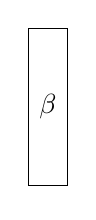
\begin{tikzpicture}[baseline=-0.5ex]
    \draw (0,0) rectangle (.5,2) node[pos=.5] {$\beta$};
\end{tikzpicture}}}
=
\vcenter{\hbox{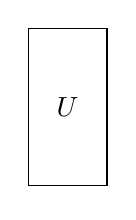
\begin{tikzpicture}[baseline=-0.5ex]
    \draw (0,0) rectangle (1,2) node[pos=.5] {$U$};
\end{tikzpicture}}}
\times
\left(\,
\vcenter{\hbox{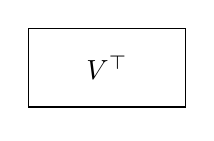
\begin{tikzpicture}[baseline=-0.5ex]
    \draw (0,0) rectangle (2,1) node[pos=.5] {$V^\top$};
\end{tikzpicture}}}
\times
\vcenter{\hbox{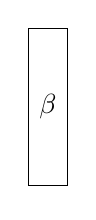
\begin{tikzpicture}[baseline=-0.5ex]
    \draw (0,0) rectangle (.5,2) node[pos=.5] {$\beta$};
\end{tikzpicture}}}
\,\right)
\]
resulting in two matrix-vector products of cost $O(ZR)$ each
\end{frame}

\begin{frame}
\frametitle{Hypergraph Marginalization}
\begin{itemize}
\item 
\end{itemize}
\end{frame}

\begin{frame}
\frametitle{Hypergraph Marginalization Algorithm}

\end{frame}


\section{Experiments}

\begin{frame}
\frametitle{Experiments}
\begin{itemize}
\item Language modeling on PTB
\vspace{2em}
\item Feature map $\phi(U) = \exp\left(U W\right)$,
with learned $W\in\R^{R \times R}$
\vspace{2em}
\item Baseline: Softmax HMM
\end{itemize}
\end{frame}

\begin{frame}
\frametitle{HMM Accuracy}
\centering
\begin{tabular}{lrr}
\toprule
Model & Val & Test\\

\midrule
%AWD-LSTM-DOC & 54.1 & 52.4\\
AWD-LSTM & 60.0 & 57.3\\
VL-HMM & 128.6 & 119.5\\
HMM & 144.3 & 136.8\\
LHMM & 141.4 & 131.8\\
\bottomrule
\end{tabular}
\end{frame}

\begin{frame}
\frametitle{HMM Speed vs Accuracy Frontier}
\end{frame}

\begin{frame}
\frametitle{HMM Accuracy vs Rank}
\begin{center}
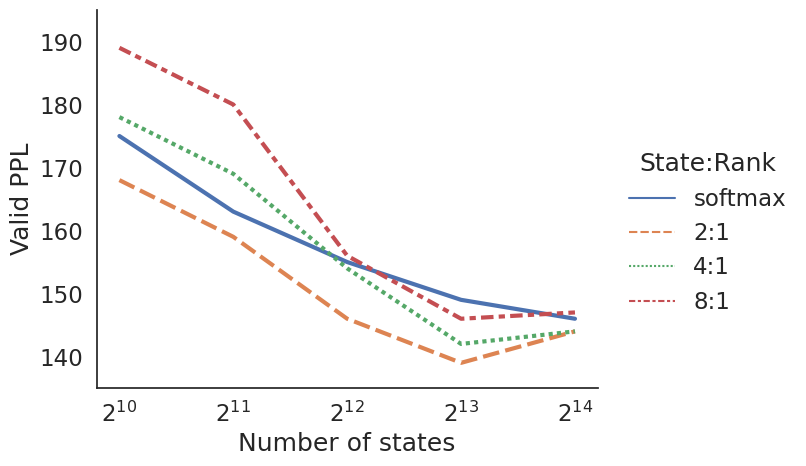
\includegraphics[height=5cm]{imgs/hmm/lhmm-states-features-dropout.png}
\end{center}
\end{frame}

\begin{frame}
\frametitle{HMM Speed vs Rank}
\begin{center}
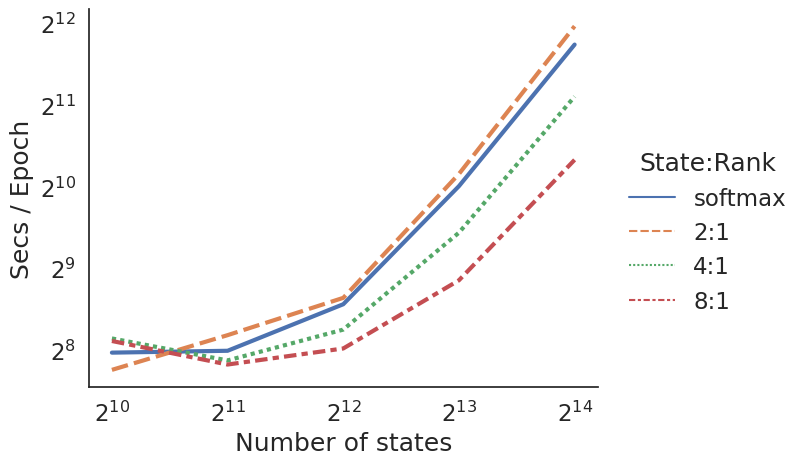
\includegraphics[height=5cm]{imgs/hmm/lhmm-states-features-speed.png}
\end{center}
\end{frame}

\begin{frame}
\frametitle{HMM Music Results}
\centering
\begin{tabular}{lrrrr}
\toprule
Model       & Nott & Piano & Muse & JSB \\
\midrule
%RNN      & 4.46       & 8.37        & 8.13       & 8.71          \\ 
%\midrule 
RNN-NADE & 2.31  & \textbf{7.05}        & \textbf{5.6}        & 5.19          \\
%\midrule
R-Transformer & \textbf{2.24} & 7.44 & 7.00 & 8.26 \\
LSTM  & 3.43 & 7.77   & 7.23 & 8.17     \\
%\midrule
LV-RNN    & 2.72       & 7.61        & 6.89       &\textbf{ 3.99}\\
SRNN     & 2.94       & 8.20         & 6.28       & 4.74          \\
\midrule
TSBN     & 3.67       & 7.89        & 6.81       & 7.48          \\
HMM &  2.43 & 8.51 & 7.34 & 5.74 \\
LHMM & 2.60 & 8.89 & 7.60 & 5.80 \\
\bottomrule
\end{tabular}
\end{frame}

\begin{frame}
\frametitle{PCFG Results}
\centering
\begin{tabular} {lllrrrr}
\toprule
$|\mathcal{N}|$ & $|\mathcal{P}|$ & Model & $N$ &  PPL & Batch/s\\
\midrule
30  & 60    & PCFG & - & 252.60 & 4.37\\
    &       & LPCFG & 8 &  247.02    & 3.75\\
    &       & LPCFG & 16 & 250.59    & 3.74\\
\midrule
60  & 120   & PCFG & - & 234.01 & 2.99\\
    &       & LPCFG & 16& 217.24 & 3.55\\
    &       & LPCFG & 32& 213.81 & 3.35\\
\midrule
100 & 200   & PCFG & - &  191.08   & 0.98\\
    &       & LPCFG & 32& 203.47 & 1.56\\
    &       & LPCFG & 64& 194.25 & 1.24\\
\bottomrule
\end{tabular}
\end{frame}

\begin{frame}
\frametitle{HSMM Results}
\centering
\begin{tabular} {lllrrrr}
\toprule
Model & $L$ & $N$ & NLL & Batch/s \\
\midrule
HSMM & $2^6$ & - & $1.428e5$ & 1.28 \\
HSMM & $2^7$ & - & $1.427e5$  & 0.45\\
HSMM & $2^8$ & - & $1.426e5$ & 0.13 \\
\midrule
LHSMM & $2^7$ & $2^7$ & $1.427e5$ & 0.24 \\
LHSMM & $2^8$ & $2^6$ & $1.426e5$ & 0.20 \\
LHSMM & $2^9$ & $2^5$ & $1.424e5$ & 0.18 \\
LHSMM & $2^{10}$ & $2^4$ & $1.423e5$ & 0.10 \\
\bottomrule
\end{tabular}
\end{frame}


\begin{frame}
\frametitle{Citations}
\printbibliography
\end{frame}



\end{document}
